\part{Complex-Numbers-II}
\lecture{Complex Numbers II}{Complex-Numbers-II}
\section{Complex Numbers II}

\title{Ordinary Differential Equations}
\subtitle{Math 232 - Week 5, Day 1}
\date{21 Sep 2012}

\begin{frame}
  \titlepage
\end{frame}

\begin{frame}
  \frametitle{Outline}
  \tableofcontents[pausesection,hideothersubsections]
\end{frame}

\subsection{Euler's Formula}
\begin{frame}
  \frametitle{Euler's Formula}

  \begin{eqnarray*}
    e^{it} & = & \cos(t) + i\sin(t)\\
    e^{i\theta} & = & \cos(\theta) + i\sin(\theta)
  \end{eqnarray*}

  Different format of a complex number:
    \begin{eqnarray*}
    z & = & a + bi, \\
    & = & r\cos(\theta) + ir\sin(\theta), ~ r = \sqrt{a^2+b^2}, \tan(\theta)=\frac{b}{a} \\
    & = & r \lp \cos(\theta) + i\sin(\theta) \rp \\
    & = & r e^{i\theta}
  \end{eqnarray*}

\end{frame}


\begin{frame}
  \frametitle{Example}

  \begin{eqnarray*}
    z & = & 2 + 2i \\
    \uncover<2->
    {%
       & = & 2\sqrt{2} \cos(\pi/4) + i 2\sqrt{2} \sin(\pi/4) \\
       & = & 2\sqrt{2} \lp \cos(\pi/4) + i\sin(pi/4) \rp \\
       & = & 2\sqrt{2} e^{i\pi/4}
    }
  \end{eqnarray*}
\end{frame}

\begin{frame}
  \frametitle{Example}
  \begin{eqnarray*}
    z & = & \sqrt{3} + i \\
    \uncover<2->
    {%
         & = & 2 \cos\lp\frac{\pi}{6}\rp + i 2 \sin\lp\frac{\pi}{6}\rp, \\
         & = & 2 e^{i\frac{\pi}{6}}.
    }
  \end{eqnarray*}
\end{frame}

\iftoggle{clicker}{%
\begin{frame}
  \frametitle{Clicker Quiz}

      \ifnum\value{clickerQuiz}=1{%

        Express -1 in Euler form.

          \begin{tabular}{l@{\hspace{3em}}l}
            A: & $e^{-i\pi}$, \\
            B: & $e^{-i\pi/2}$, \\
            C: & $e^{-i}$, \\
            D: & $-1$, \\
          \end{tabular}

     }\fi

     \ifnum\value{clickerQuiz}=2{%

        Express -1 in Euler form.

          \begin{tabular}{l@{\hspace{3em}}l}
            A: & $e^{-i\pi}$, \\
            B: & $e^{-i\pi/2}$, \\
            C: & $e^{-i}$, \\
            D: & $-1$, \\
          \end{tabular}


     }\fi

      \ifnum\value{clickerQuiz}=3{%
         Express -1 in Euler form.

          \begin{tabular}{l@{\hspace{3em}}l}
            A: & $e^{-i\pi}$, \\
            B: & $e^{-i\pi/2}$, \\
            C: & $e^{-i}$, \\
            D: & $-1$, \\
          \end{tabular}

     }\fi

    \vfill
    \vfill
    \vfill

\end{frame}

}

\subsection{Root Finding}

\begin{frame}
  \frametitle{So What?}

  What is the cube root of 1?
  \begin{eqnarray*}
    \uncover<2->{1,~e^{i2\pi/3},~e^{i4\pi/3}}.
  \end{eqnarray*}

  \uncover<3->
  {
    Cuz....
    \begin{eqnarray*}
      1^3 & = & 1. \\
      \lp e^{i2\pi/3} \rp^3 & = &  e^{i2\pi} \\
      \lp e^{i4\pi/3} \rp^3 & = & e^{i4\pi}
    \end{eqnarray*}


  }

  
\end{frame}

\begin{frame}
  \frametitle{Cube Root of One}
  \centerline{\includegraphics[width=6cm]{img/cubeRoot}}
\end{frame}



\begin{frame}
  \frametitle{lol wut?}

  Find the cube roots of 3.
  \begin{eqnarray*}
    z^3 & = & 1 \\
    z^3 & = & \lp r e^{i\theta} \rp^3 \\
    z^3 & = & r^3 e^{i3\theta}
  \end{eqnarray*}

  There are three ways to express the number ``1''
  \begin{eqnarray*}
    z^3 & = & e^{i0} \\
    z^3 & = & e^{i2\pi} \\
    z^3 & = & e^{i4\pi}
  \end{eqnarray*}
  
  % TODO - add a picture of the point in the complex plane
\end{frame}

\begin{frame}
  \frametitle{Root Finding}
  To find the n\textsuperscript{th} roots:
  \begin{itemize}
  \item n\textsuperscript{th} roots of $a+bi$
  \item Convert $a+bi=re^{i\theta}$ 
  \item Find $z^n=re^{i\theta}$
    \begin{eqnarray*}
      z^n & = & re^{i\theta} \\
      z^n & = & re^{i(\theta+2\pi)} \\
      z^n & = & re^{i(\theta+4\pi)} \\
      z^n & = & re^{i(\theta+6\pi)} \\
      \vdots & & \vdots \\
      z^n & = & re^{i(\theta+2(n-1)\pi)} \\
    \end{eqnarray*}
  \end{itemize}
\end{frame}

\begin{frame}
  If 
  \begin{eqnarray*}
    z & = & R e^{i\alpha} \\
    z^n & = & R^n e^{i n\alpha} \\
  \end{eqnarray*}
  but
  \begin{eqnarray*}
    z^n & = & re^{i\theta}, \\
    \uncover<2->{%
      \Rightarrow
      R & = & r^{1/n} \\
      \alpha & = & \frac{\theta}{n}, ~ \frac{\theta+2\pi}{n}, ~
      \frac{\theta+4\pi}{n}, \ldots, ~ \frac{\theta+2(n-1)\pi}{n}.
    }
  \end{eqnarray*}
\end{frame}

\begin{frame}
  \frametitle{Example}

  Find the fourth roots of 16.
  \only<2->{%
    Express 16 four different ways:
    \begin{eqnarray*}
      z & = & R e^{i\alpha}, \\
      z^4 & = & 16 e^{i0}, ~ 16 e^{i2\pi}, ~ 16 e^{i4\pi}, ~ 16 e^{i6\pi} \\
      R^4 e^{i4\alpha} & = & 16 e^{i0}, ~ 16 e^{i2\pi}, ~ 16 e^{i4\pi}, ~ 16 e^{i6\pi} 
    \end{eqnarray*}
  }

  \only<3->{%
    Then
    \begin{eqnarray*}
      R & = & 2 \\
      \alpha & = & 0, ~ \frac{\pi}{2}, ~ \pi, ~ \frac{3\pi}{2}
    \end{eqnarray*}
  }

  \only<4->{%
    \begin{eqnarray*}
      z & = & 2 e^{i0},~2e^{i\pi/2},~2e^{i\pi},~2e^{i3\pi/2}, \\
      & = & 2,~2i,~-2,~-2i.
    \end{eqnarray*}
  }

\end{frame}



\begin{frame}
  \frametitle{Example}

  Find the cubic roots of $2+2i$.

  \uncover<2->{%
    \begin{eqnarray*}
      2 + 2i & = & 2\sqrt{2} e^{i\pi/4}
    \end{eqnarray*}

    Let $z=re^{i\theta}$ so $z^3=r^3e^{i3\theta}$:
    \begin{eqnarray*}
      r^3e^{i3\theta} & = & 2\sqrt{2} e^{i\pi/4}, ~ 2\sqrt{2} e^{i9\pi/4}, ~ 2\sqrt{2} e^{i17\pi/4}
    \end{eqnarray*}

    \begin{eqnarray*}
      r &  = & (2\sqrt{2})^{1/3} \\
      \theta & = & \frac{\pi}{12}, ~ \frac{9\pi}{12}, ~ \frac{17\pi}{12} \\
      z & = &  (2\sqrt{2})^{1/3} e^{i\pi/12}, ~ (2\sqrt{2})^{1/3} e^{i9\pi/12}, ~ (2\sqrt{2})^{1/3} e^{i17\pi/12}
    \end{eqnarray*}

  }

\end{frame}



\iftoggle{clicker}{%
\begin{frame}
  \frametitle{Clicker Quiz}
    
      \ifnum\value{clickerQuiz}=1{%

        \vfill

        Determine the square roots of $\sqrt{3}+i$

        \vfill

        %\begin{eqnarray*}
        %  \sqrt{3} + i & = & 2 e^{\pi/6} 
        %\end{eqnarray*}

        %Let $z=re^{i\theta}$ so $z^2=r^2e^{i2\theta}$:
        %\begin{eqnarray*}
        %  r^2e^{i2\theta} & = & 2 e^{\pi/6} , ~ 2 e^{13\pi/6} 
        %\end{eqnarray*}

        %\begin{eqnarray*}
        %  r & = & \sqrt{2} \\
        %  \theta & = & \frac{\pi}{12}, ~ \frac{13\pi}{12}
        %\end{eqnarray*}

          \begin{tabular}{l@{\hspace{3em}}l@{\hspace{1em}}l}
            A: &  $\sqrt{2}e^{i\frac{\pi}{12}}$, & $\sqrt{2} e^{i\frac{13\pi}{12}}$ \\
            B: &  $\sqrt{2}e^{i\frac{\pi}{6}}$, & $\sqrt{2}e^{i\frac{13\pi}{6}}$ \\
            C: &  $2e^{i\frac{\pi}{12}}$, & $2e^{i\frac{13\pi}{12}}$ \\
            D: &  $2e^{i\frac{\pi}{6}}$, & $2e^{i\frac{13\pi}{6}}$ \\ 
          \end{tabular}

          \vfill

     }\fi

     \ifnum\value{clickerQuiz}=2{%

       \vfill

        Determine the square roots of $1 + \sqrt{3}i$

        \vfill 

        %\begin{eqnarray*}
        %  1 + \sqrt{3} i & = & 2 e^{\pi/3} 
        %\end{eqnarray*}

        %Let $z=re^{i\theta}$ so $z^2=r^2e^{i2\theta}$:
        %\begin{eqnarray*}
        %  r^2e^{i2\theta} & = & 2 e^{\pi/3} , ~ 2 e^{7\pi/3} 
        %\end{eqnarray*}

        %\begin{eqnarray*}
        %  r & = & \sqrt{2} \\
        %  \theta & = & \frac{\pi}{6}, ~ \frac{7\pi}{6}
        %\end{eqnarray*}


        \begin{tabular}{l@{\hspace{3em}}l@{\hspace{1em}}l}
          A: &  $\sqrt{2}e^{i\frac{\pi}{3}}$, & $\sqrt{2}e^{i\frac{7\pi}{3}}$ \\
          B: &  $\sqrt{2}e^{i\frac{\pi}{6}}$, & $\sqrt{2} e^{i\frac{7\pi}{6}}$ \\
          C: &  $2e^{i\frac{\pi}{3}}$, & $2e^{i\frac{7\pi}{3}}$ \\ 
          D: &  $2e^{i\frac{\pi}{6}}$, & $2e^{i\frac{7\pi}{6}}$ \\
        \end{tabular}

        \vfill


     }\fi

      \ifnum\value{clickerQuiz}=3{%
       Determine the square roots of $\sqrt{3} + i$

        \vfill

        %\begin{eqnarray*}
        %  \sqrt{3} +  i & = & 2 e^{\pi/6} 
        %\end{eqnarray*}

        %Let $z=re^{i\theta}$ so $z^2=r^2e^{i2\theta}$:
        %\begin{eqnarray*}
        %  r^2e^{i2\theta} & = & 2 e^{\pi/6} , ~ 2 e^{13\pi/6} 
        %\end{eqnarray*}

        %\begin{eqnarray*}
        %  r & = & \sqrt{2} \\
        %  \theta & = & \frac{\pi}{6}, ~ \frac{13\pi}{6}
        %\end{eqnarray*}


        \begin{tabular}{l@{\hspace{3em}}l@{\hspace{1em}}l}
          A: &  $\sqrt{2}e^{i\frac{\pi}{3}}$, & $\sqrt{2}e^{i\frac{7\pi}{3}}$ \\
          B: &  $\sqrt{2}e^{i\frac{\pi}{6}}$, & $\sqrt{2} e^{i\frac{13\pi}{6}}$ \\
          C: &  $2e^{i\frac{\pi}{3}}$, & $2e^{i\frac{7\pi}{3}}$ \\
          D: &  $2e^{i\frac{\pi}{6}}$, & $2e^{i\frac{13\pi}{6}}$ \\
        \end{tabular}

     }\fi

    \vfill
    \vfill
    \vfill

\end{frame}

}


\begin{frame}
  \frametitle{Important Properties}

  Euler's Formula
  \begin{eqnarray*}
    e^{it} & = & \cos(t) + i\sin(t). 
  \end{eqnarray*}

  Note:
  \begin{eqnarray*}
    e^{-it} & = & \cos(-t) + i\sin(-t) \\
    & = & \cos(t) - i\sin(t)
  \end{eqnarray*}

  So...
  \begin{eqnarray*}
    e^{it} + e^{-it} & = & 2 \cos(t), \\
    \frac{e^{it} + e^{-it}}{2} & = & \cos(t).
  \end{eqnarray*}

  Also,
  \begin{eqnarray*}
    e^{it} - e^{-it} & = & 2 i \sin(t), \\
    \frac{e^{it} - e^{-it}}{2i} & = & \sin(t).
  \end{eqnarray*}



\end{frame}


\begin{frame}
  \frametitle{Quick Example}

  \begin{eqnarray*}
    \cos(3t) & = & \frac{e^{i3t}+e^{-i3t}}{2} \\
    \sin(4t) & = & \frac{e^{i4t}-e^{-i4t}}{2i}
  \end{eqnarray*}

\end{frame}


\begin{frame}
  \frametitle{Another thing...}

  \begin{eqnarray*}
    e^{a+ib} & = & e^a e^{ib} \\
    & = & e^a \lp \cos(b) + i \sin(b) \rp.
  \end{eqnarray*}

  Thusly...
  \begin{eqnarray*}
    e^{a-ib} & = & e^a \lp \cos(b) - i \sin(b) \rp.
  \end{eqnarray*}

\end{frame}


\begin{frame}
  \frametitle{What do we have here?}

  \begin{eqnarray*}
    e^a \cos(b) & = & e^a \lp \frac{e^{ib}+e^{-ib}}{2} \rp \\
    & = & \half e^a e^{ib} +\half e^a  e^{-ib} \\
    e^a \sin(b) & = & e^a \lp \frac{e^{ib}-e^{-ib}}{2i} \rp \\
    & = & \frac{1}{2i} e^a e^{ib} - \frac{1}{2i} e^a e^{-ib}
  \end{eqnarray*}

\end{frame}

\subsection{Derivatives and Integrals}

\begin{frame}
  \frametitle{Derivatives and Integrals}

  \begin{eqnarray*}
    f(t) & = & u(t) + i v(t) \\
    f'(t) & = & u'(t) + i v'(t),
  \end{eqnarray*}

  and
  \begin{eqnarray*}
    \int f(t) ~ dt & = & \int u(t) + i v(t) ~ dt, \\
    & = & \int u(t) ~ dt + i \int v(t) ~ dt.
  \end{eqnarray*}

\end{frame}


\begin{frame}
  \frametitle{Examples}

  \begin{eqnarray*}
    \frac{d}{dt} \lp \sin(t) + i e^{2t} \cos(t) \rp & = & 
    \cos(t) + i \lp 2 e^{2t} \cos(t) - e^{2t} \sin(t) \rp.
  \end{eqnarray*}

  \begin{eqnarray*}
    \int \sin(t) + i t \cos(t) ~ dt & = & 
    \int \sin(t) ~ dt + i \int t \cos(t) ~ dt \\
    & = & \cos(t) + i \lp t\sin(t) + \cos(t) \rp + C
  \end{eqnarray*}

  Note that ``$C$'' is a complex number!
  \begin{eqnarray*}
    C & = & C_1 + i C_2.
  \end{eqnarray*}

\end{frame}

\subsection{What does this have to do with DEs?}

\begin{frame}
  \frametitle{Why do we care?}

  Show that $y=C_1 e^{(-3+i)t} + C_2 e^{(-3-i)t}$ is a solution to the DE
  \begin{eqnarray*}
    y'' + 6y' + 10y & = & 0.
  \end{eqnarray*}

\end{frame}




% LocalWords:  Clarkson pausesection hideothersubsections
